\documentclass{article}
\usepackage[utf8]{inputenc}
\usepackage{amsmath,amssymb}
\usepackage{graphicx}
\usepackage{float}
\usepackage{subcaption}
\usepackage{geometry}
\geometry{
    a4paper,
    total={170mm,257mm},
    left=20mm,
    right=20mm,
    top=20mm,
}
\usepackage{listings} % code listings
\lstset{framextopmargin=0pt,frame=lines}
\lstset{
    language=Matlab,
    basicstyle=\footnotesize\ttfamily,
    breaklines=true,
    tabsize=4,
    keepspaces=true,
    columns=flexible,
    % backgroundcolor=\color[gray]{0.9},
    frame=single,
    breaklines=true,%
    morekeywords={matlab2tikz},
    keywordstyle=\color{blue},%
    morekeywords=[2]{1}, keywordstyle=[2]{\color{black}},
    identifierstyle=\color{black},%
    stringstyle=\color{mylilas},
    commentstyle=\color{mygreen},%
    showstringspaces=false,%without this there will be a symbol in the places where there is a space
    numbers=left,
    numberstyle={\tiny \color{black}},% size of the numbers
    numbersep=9pt, % this defines how far the numbers are from the text
    emph=[1]{for,end,break},emphstyle=[1]\color{red}, %some words to emphasise
    %emph=[2]{word1,word2}, emphstyle=[2]{style},
}
\usepackage{color} %red, green, blue, yellow, cyan, magenta, black, white
\definecolor{mygreen}{RGB}{28,172,0} % color values Red, Green, Blue
\definecolor{mylilas}{RGB}{170,55,241}

\usepackage{siunitx}
\newcommand{\e}[1]{\times 10^{#1}} % nicer scientific notation

\title{ENV-541 Sensor Orientation\\Lab 8 - Kalman Filtering with simulated GPS data: constant acceleration (a = const.) model}
\author{Michael Spieler}
\date{November 23, 2018}

\begin{document}

\maketitle

\section*{Plots}

Figure \ref{fig:traj} compares the true trajectory with the noisy GPS measurments and the estimated position for one realizations.

\begin{figure}[H]
    \centering
    \begin{subfigure}[t]{0.8\textwidth}
        \centering
        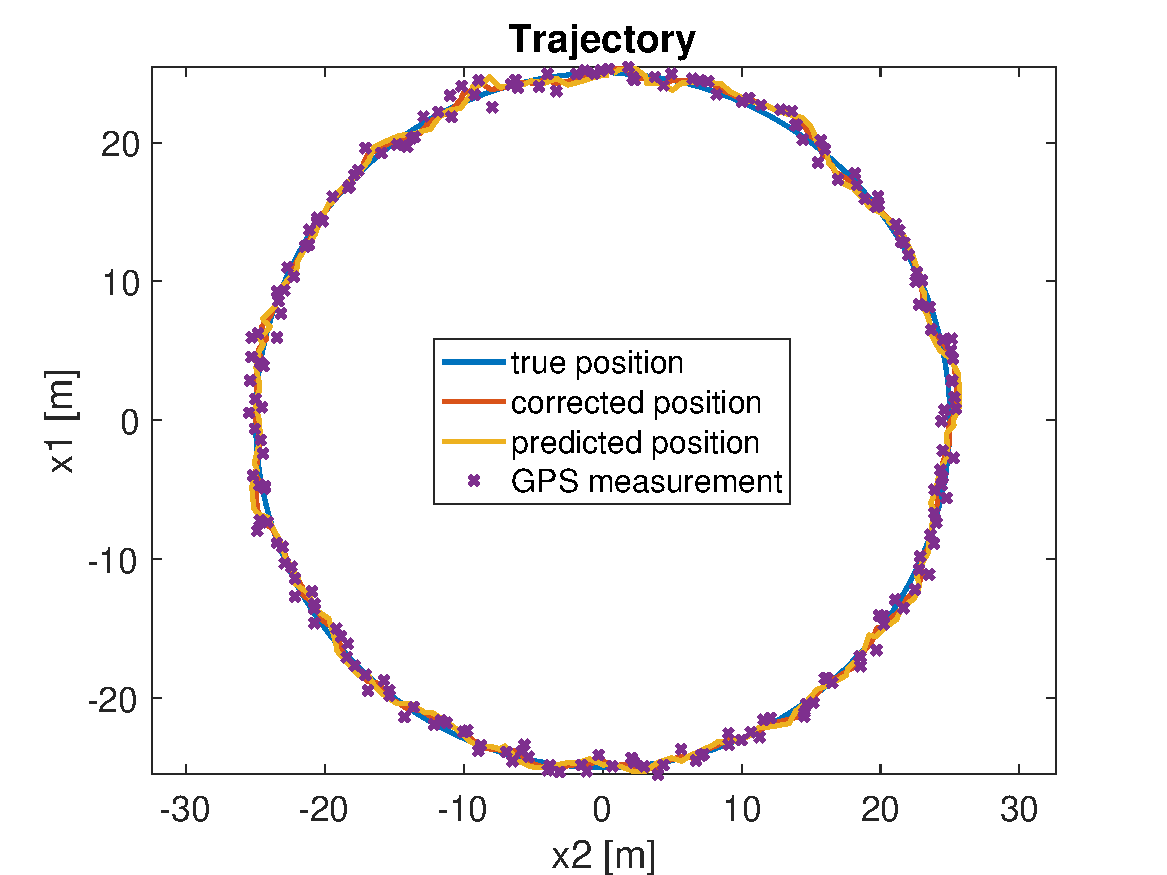
\includegraphics[width=\textwidth]{traj}
    \end{subfigure}
    \caption{Trajectory compared with measurements and KF estimate.}
    \label{fig:traj}
\end{figure}


\begin{figure}[H]
    \centering
    \begin{subfigure}[t]{0.49\textwidth}
        \centering
        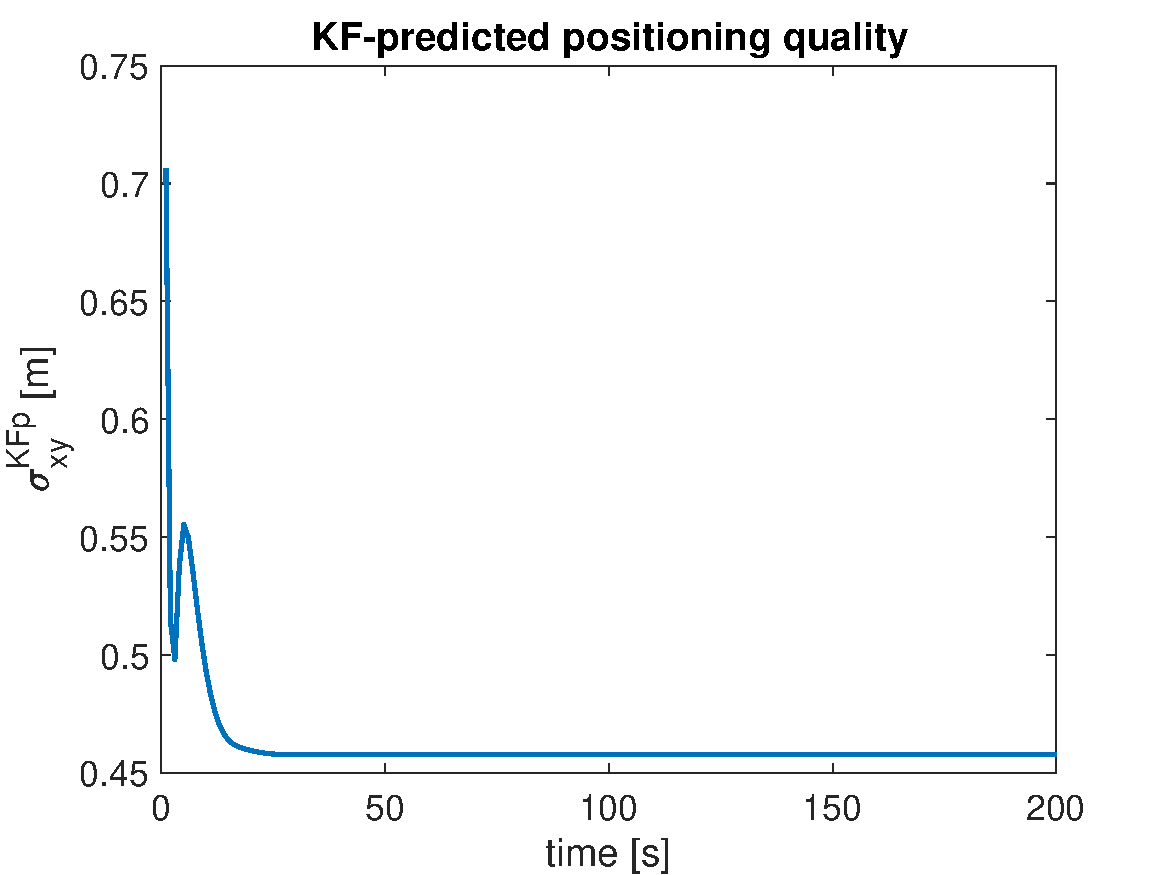
\includegraphics[width=\textwidth]{dt1/sigma_KFp}
        \caption{$dt_{KF} = 1$}
    \end{subfigure}
    ~
    \begin{subfigure}[t]{0.49\textwidth}
        \centering
        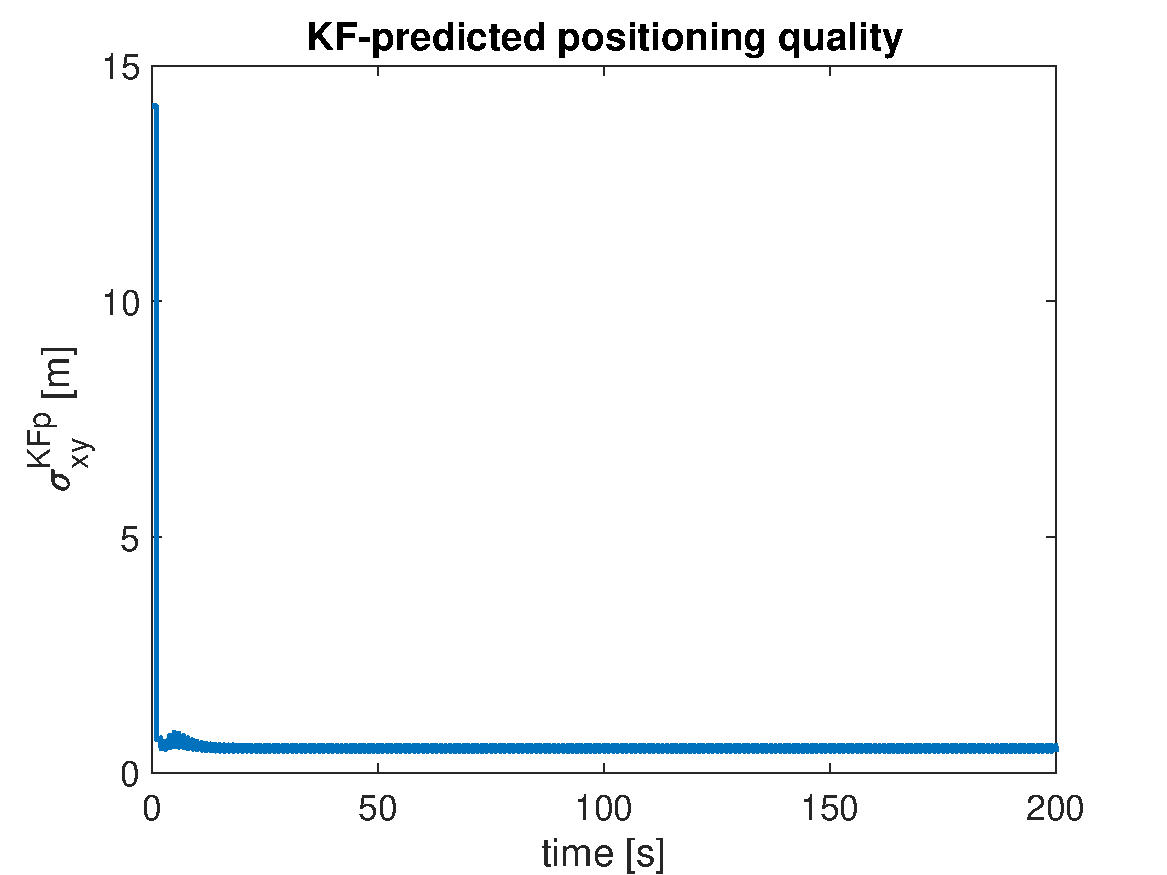
\includegraphics[width=\textwidth]{dt01/sigma_KFp}
        \caption{$dt_{KF} = 0.1$}
    \end{subfigure}
    ~
    \begin{subfigure}[t]{0.49\textwidth}
        \centering
        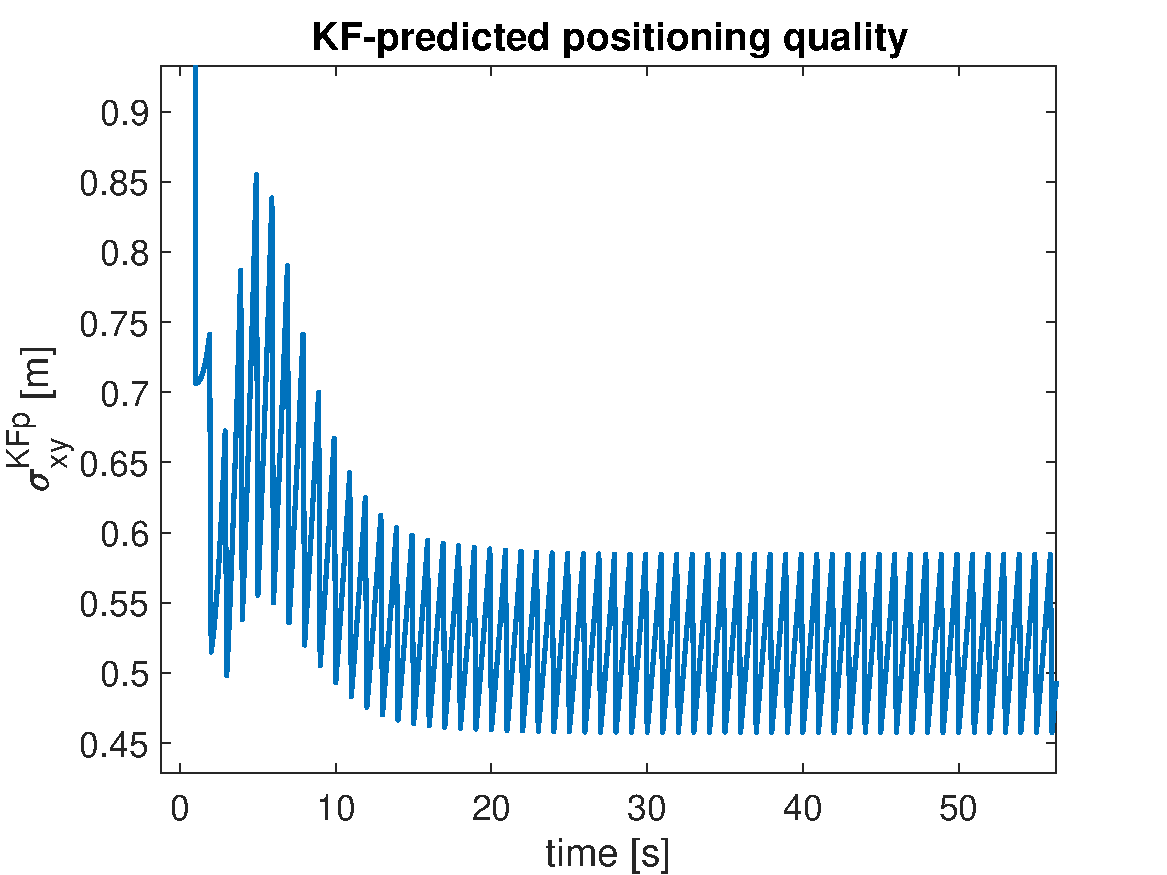
\includegraphics[width=\textwidth]{dt01/sigma_KFp_zoom}
        \caption{$dt_{KF} = 0.1$ (zoomed)}
    \end{subfigure}
    \caption{The evolution of the KF standard deviation in position $\sigma_{xy}^{KF_{p}}$}
    \label{fig:traj_motion_noise}
\end{figure}

\begin{figure}[H]
    \begin{subfigure}[t]{0.49\textwidth}
        \centering
        \includegraphics[width=\textwidth]{dt1/innovation_all}
        \caption{$dt_{KF} = 1$}
    \end{subfigure}
    ~
    \begin{subfigure}[t]{0.49\textwidth}
        \centering
        \includegraphics[width=\textwidth]{dt01/innovation_all}
        \caption{$dt_{KF} = 0.1$}
    \end{subfigure}
    ~
    \begin{subfigure}[t]{0.49\textwidth}
        \centering
        \includegraphics[width=\textwidth]{dt1/innovation_stable}
        \caption{$dt_{KF} = 1$}
    \end{subfigure}
    ~
    \begin{subfigure}[t]{0.49\textwidth}
        \centering
        \includegraphics[width=\textwidth]{dt01/innovation_stable}
        \caption{$dt_{KF} = 0.1$}
    \end{subfigure}
    \caption{The evolution of the innovation $z^{GPS} - H\tilde x$}
    \label{fig:traj_motion_noise}
\end{figure}

% # dt=1
% Empirical std dev GPS:0.6558
% Empirical std dev KF filter:0.4176
% Final std dev KF predicted:0.4577
% # dt=0.1
% Empirical std dev KF filter:0.4660
% Final std dev KF predicted:0.4577

% # dt=1 v=const
% Empirical std dev KF filter:0.4300
% Final std dev KF predicted:0.4246
% # dt=0.1 v=const
% Empirical std dev KF filter:0.4771
% Final std dev KF predicted:0.4246

\begin{table}[h]
\centering
\begin{tabular}{lllll}
Realizations  & $dt_{KF} = 1\si{s}$ & $dt_{KF} = 0.1\si{s}$ & $dt_{KF} = 1\si{s}$ & $dt_{KF} = 1\si{s}$\\
& (a=const)& (a=const) & (v=const) & (v=const)\\
\hline
$\sigma_{xy}^{GPS_{emp.}}$ & $0.6558 \si{m}$ & $0.6558 \si{m}$ & $0.6558 \si{m}$ & $0.6558 \si{m}$ \\
$\sigma_{xy}^{KF_{emp.}}$  & $0.4176 \si{m}$ & $0.4660 \si{m}$ & $0.4300 \si{m}$ & $0.4771 \si{m}$ \\
$\sigma_{xy}^{KF_{p}}$(final) & $0.4577 \si{m}$ & $0.4577 \si{m}$ & $0.4246 \si{m}$ & $0.4246 \si{m}$
\end{tabular}
\caption{Accuracy estimates from different for same GPS measurement realization but with different filtering.}
\label{tab:std_dev}
\end{table}

\section*{Questions}

\subsubsection*{I. Is the overall improvement of the \textit{positioning accuracy} via KF filtering better with
respect to the model of constant velocity (i.e. plot/compare $\sigma_{xy}^{KF_{emp.}}$ versus $\sigma_{xy}^{GPS_{emp.}}$)?
If yes/no – what do you think is the reason?}

Yes, in both cases $dt_{KF} = 1\si{s}$ and $dt_{KF} = 0.1\si{s}$ the KF filter
with constant acceleration model performs better than the filter with
constant velocity model.

Both models are not accurate but the velocity is changing faster than the acceleration.
Therefore the assumption of constant acceleration si closer to reality.

\subsubsection*{II. Is the \textit{anticipated accuracy} ($\sigma_{xy}^{KF_{p}}$) different from that of the model of constant
velocity? Provide a justification.}

Yes, they converge to different values. This is because they also have a different noise model ($Q_w$ is different).

\subsubsection*{III. How does the \textit{distribution of velocity errors} ($v^{true} – v^{KF}$) compare to that obtained
with the constant velocity model? Can you identify and explain a pattern in these
differences for the model of constant acceleration?}

The velocity error is almost normally distributed for the constant acceleration model.
For the constant velocity model is sinusoidal, since the velocity is always "lagging" behind,
such that for one circular trajectory it makes one period.

It is obvious that the constant acceleration assumption is closer to reality than constant velocity.
Thus the error is closer to anormal distribution.

It looks like there is a higher frequency oscillation for both models.
This might be the filtered velocity oscillating around the true value.
Maybe the filter is not tuned perfectly?

\begin{figure}[H]
    \begin{subfigure}[t]{0.49\textwidth}
        \centering
        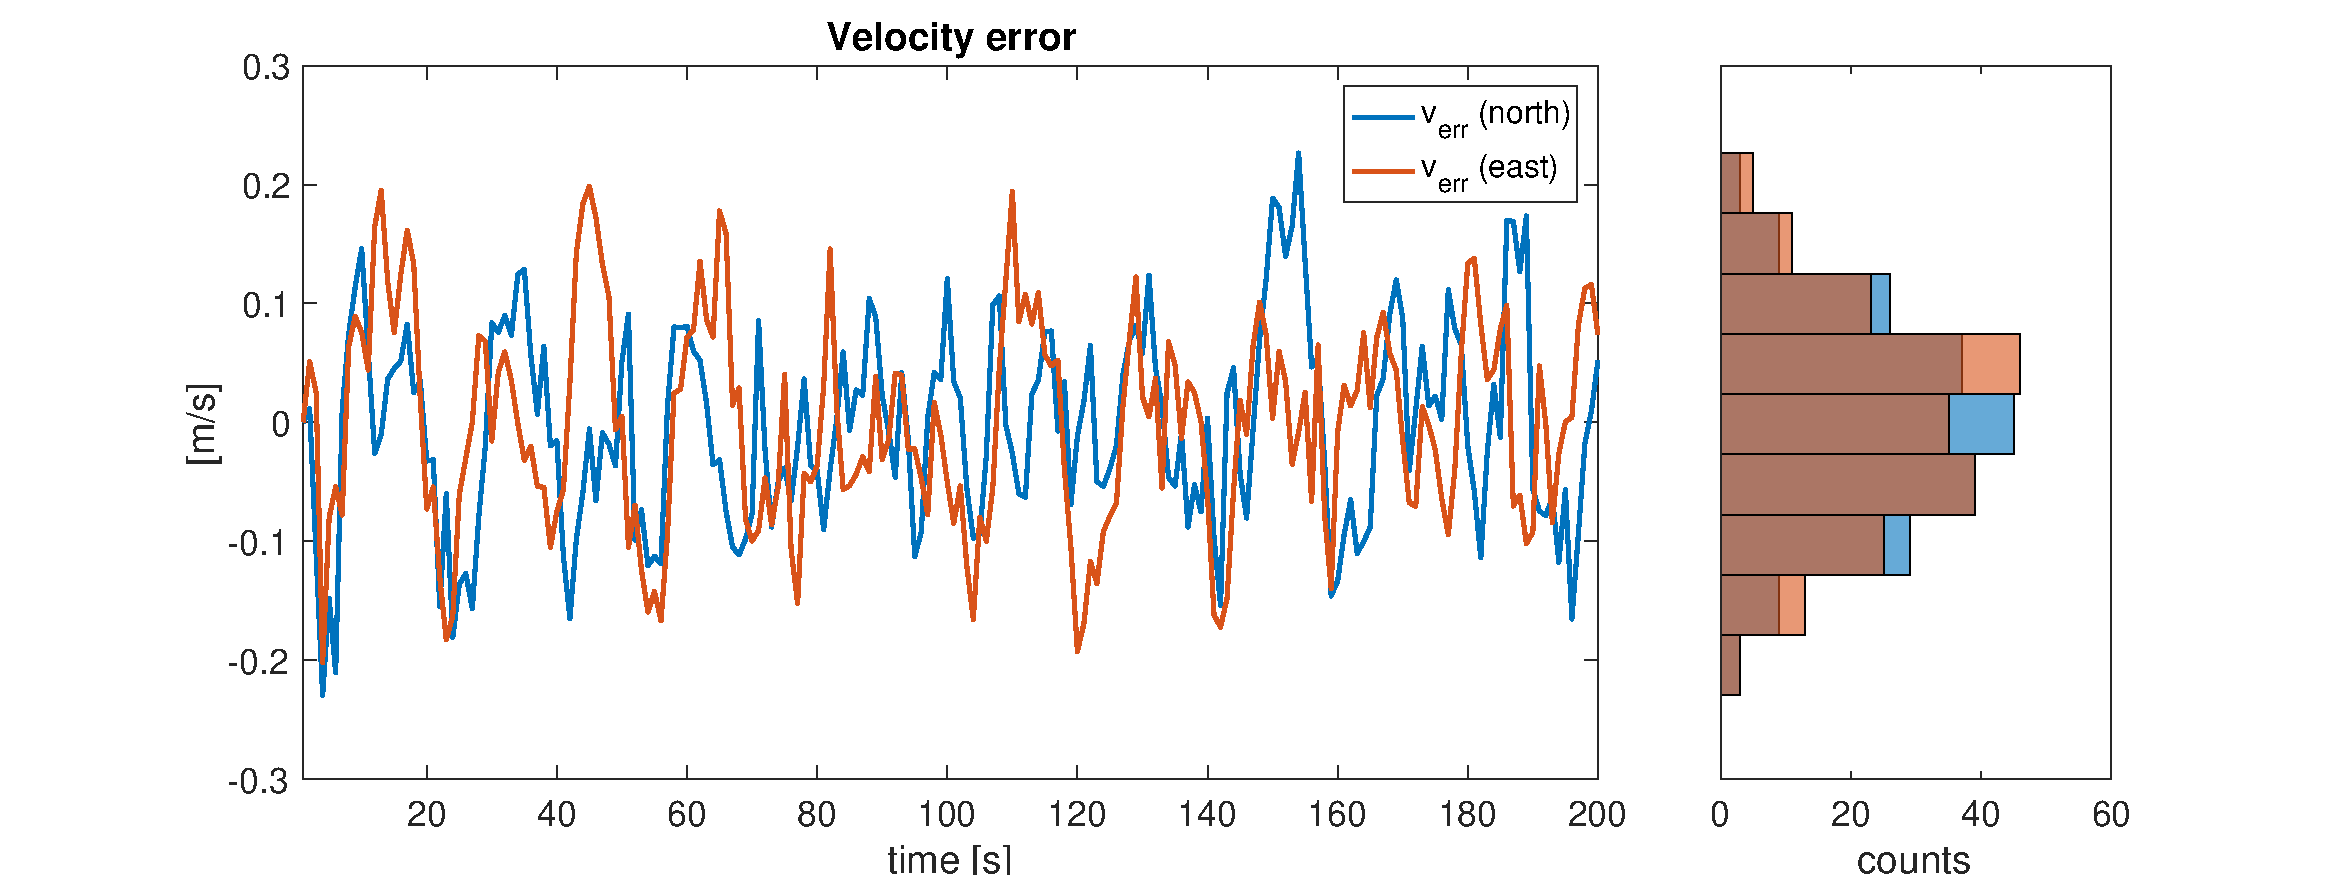
\includegraphics[width=\textwidth]{dt1/velocity_error}
        \caption{Velocity error constant acceleration model ($dt_{KF} = 1$)}
    \end{subfigure}
    ~
    \begin{subfigure}[t]{0.49\textwidth}
        \centering
        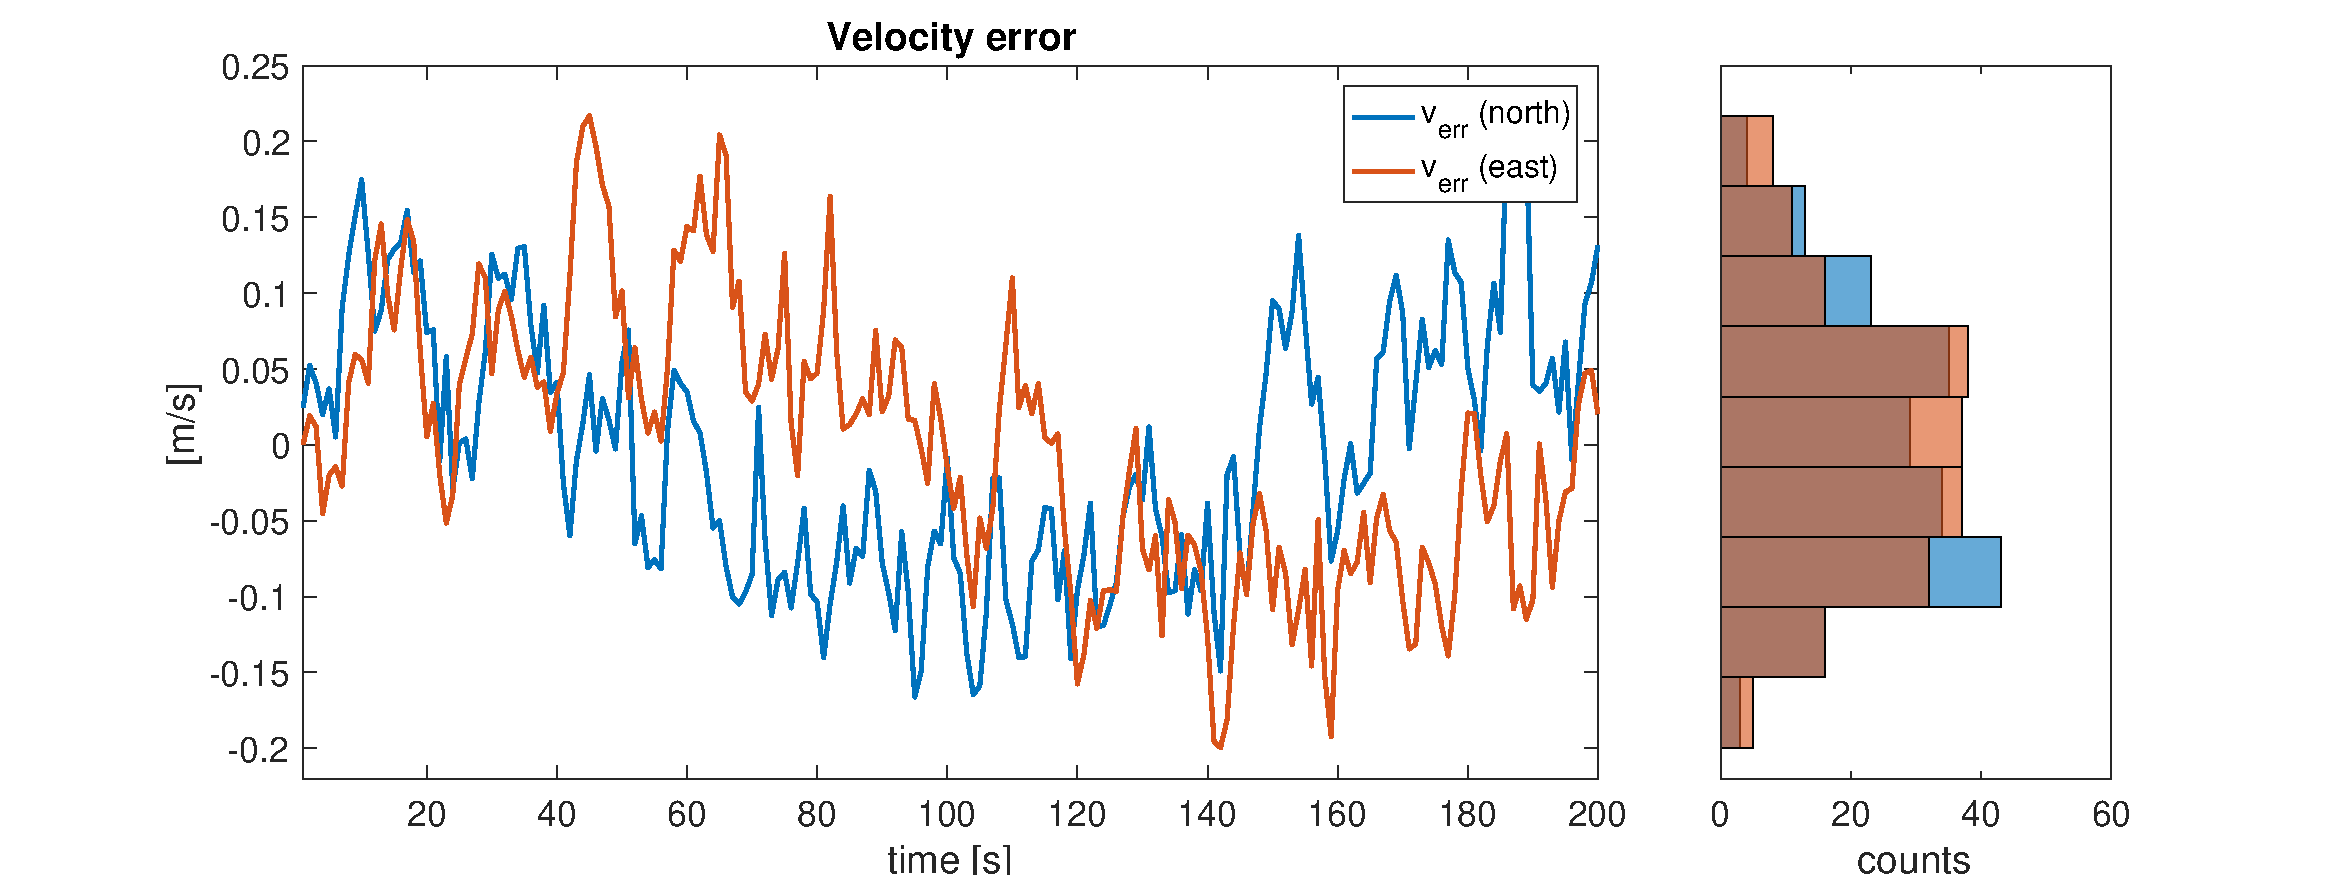
\includegraphics[width=\textwidth]{dt1vconst/velocity_error}
        \caption{Velocity error constant velocity model ($dt_{KF} = 1$)}
    \end{subfigure}
    \caption{Velocity error distribution}
    \label{fig:traj_motion_noise}
\end{figure}

\subsubsection*{IV. Do the plotted histograms of innovations look like a normal distribution (visually)?
If yes/no, which case (from A or B in Task 4.4) is closer to normality and why?}

They look both normally distributed, with B a bit closer to normality (more symmetric).
The constant acceleration model fits well the test trajectory, since the acceleration in the map frame is only changing slowly.
Therefore the position prediction noise is directly coming from the GPS gaussian noise.

Case B is better because when the gain is stabilized the covariance is lower than than at start (high initial uncertainty).
This caused the filter to give less weight to the prediciton from the motion model.

\subsubsection*{V. Do you observe statistically significant changes for the position or velocity
empirical or anticipated accuracies when using \textit{faster prediction} (i.e. $dt_{KF}=0.1s$ vs.
$dt_{KF}=1s$)? \textit{Justify} your answer by reasoning.}

The empirical velocity error distribution is almost identical for the two update frequencies.
This is reasonable, since the velocity vector will not change much by doing more prediction steps between the GPS measurement updates.

\subsubsection*{VI. Observe what happens when you first increase and then decrease the given value of
the system noise level ($\sigma_{\dot a}$) 10 times. How do you interpret the observed changes
in the filtered positions, velocities and the distribution of innovation, respectively?}

It changes the weighting between the motion model and the measurements.
If the system noise is low then the trajectory is more smooth and it only slowly follows the measurements.
However, if the system noise is high then the trajectory is very noisy, closely following the noisy measurements.

\begin{figure}[H]
    \centering
    \begin{subfigure}[t]{0.49\textwidth}
        \centering
        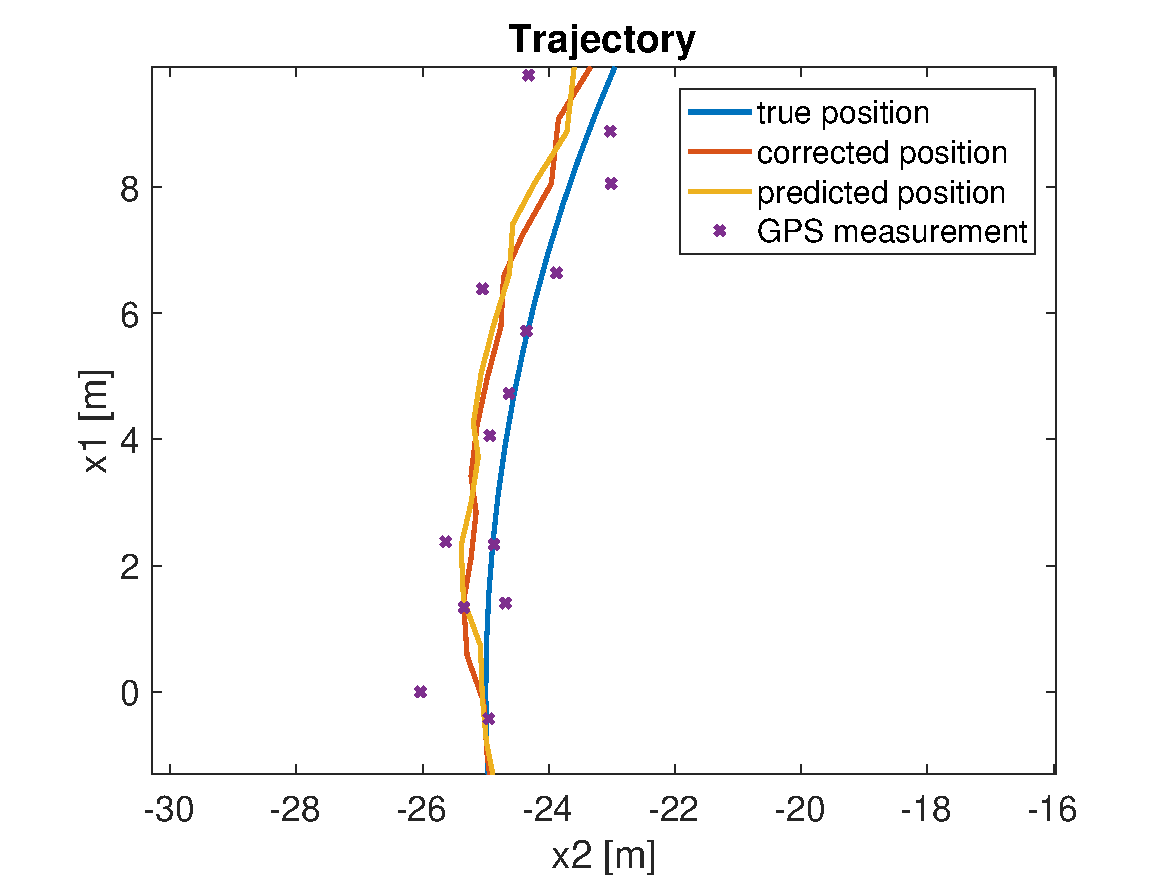
\includegraphics[width=\textwidth]{dt1_smaller_motion_noise/traj_zoom}
        \caption{trajectory 10x smaller system noise}
    \end{subfigure}
    ~
    \begin{subfigure}[t]{0.49\textwidth}
        \centering
        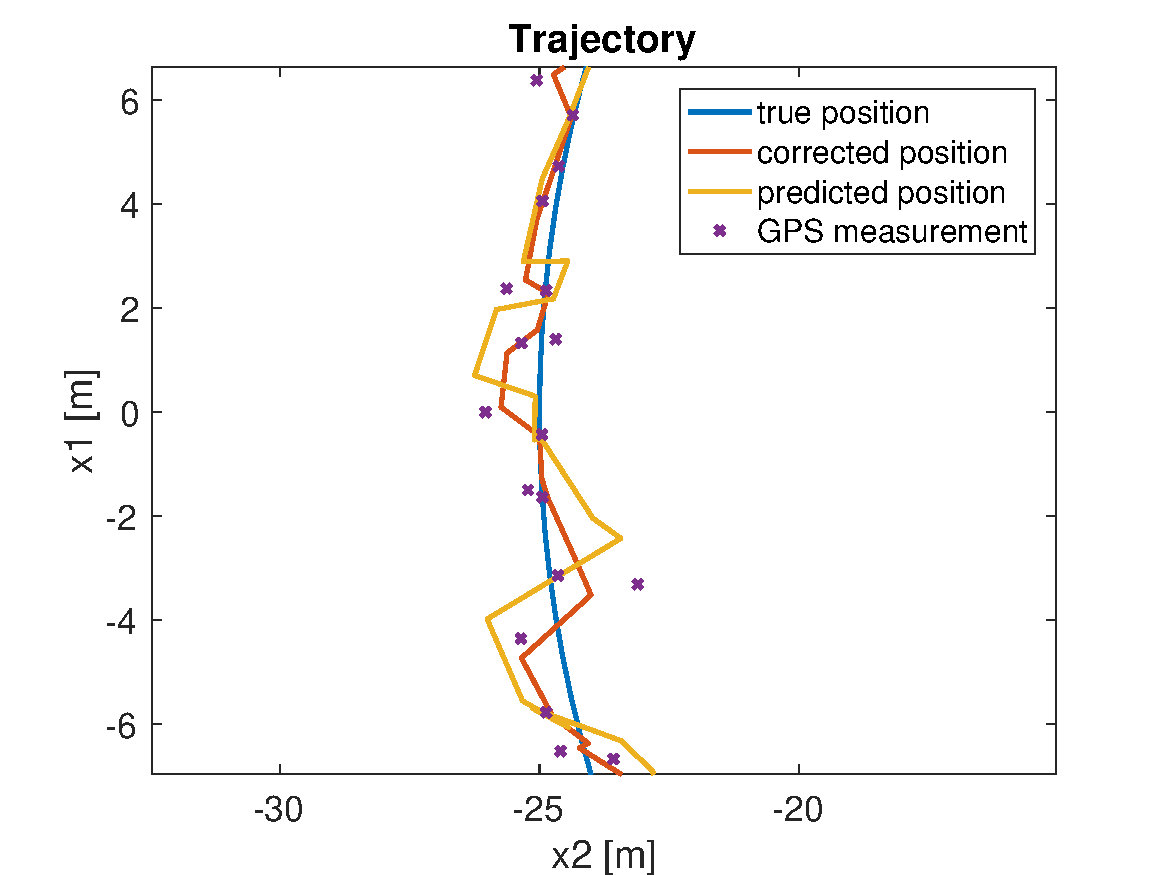
\includegraphics[width=\textwidth]{dt1_bigger_motion_noise/traj_zoom}
        \caption{trajectory 10x bigger system noise}
    \end{subfigure}
    ~
    \begin{subfigure}[t]{0.49\textwidth}
        \centering
        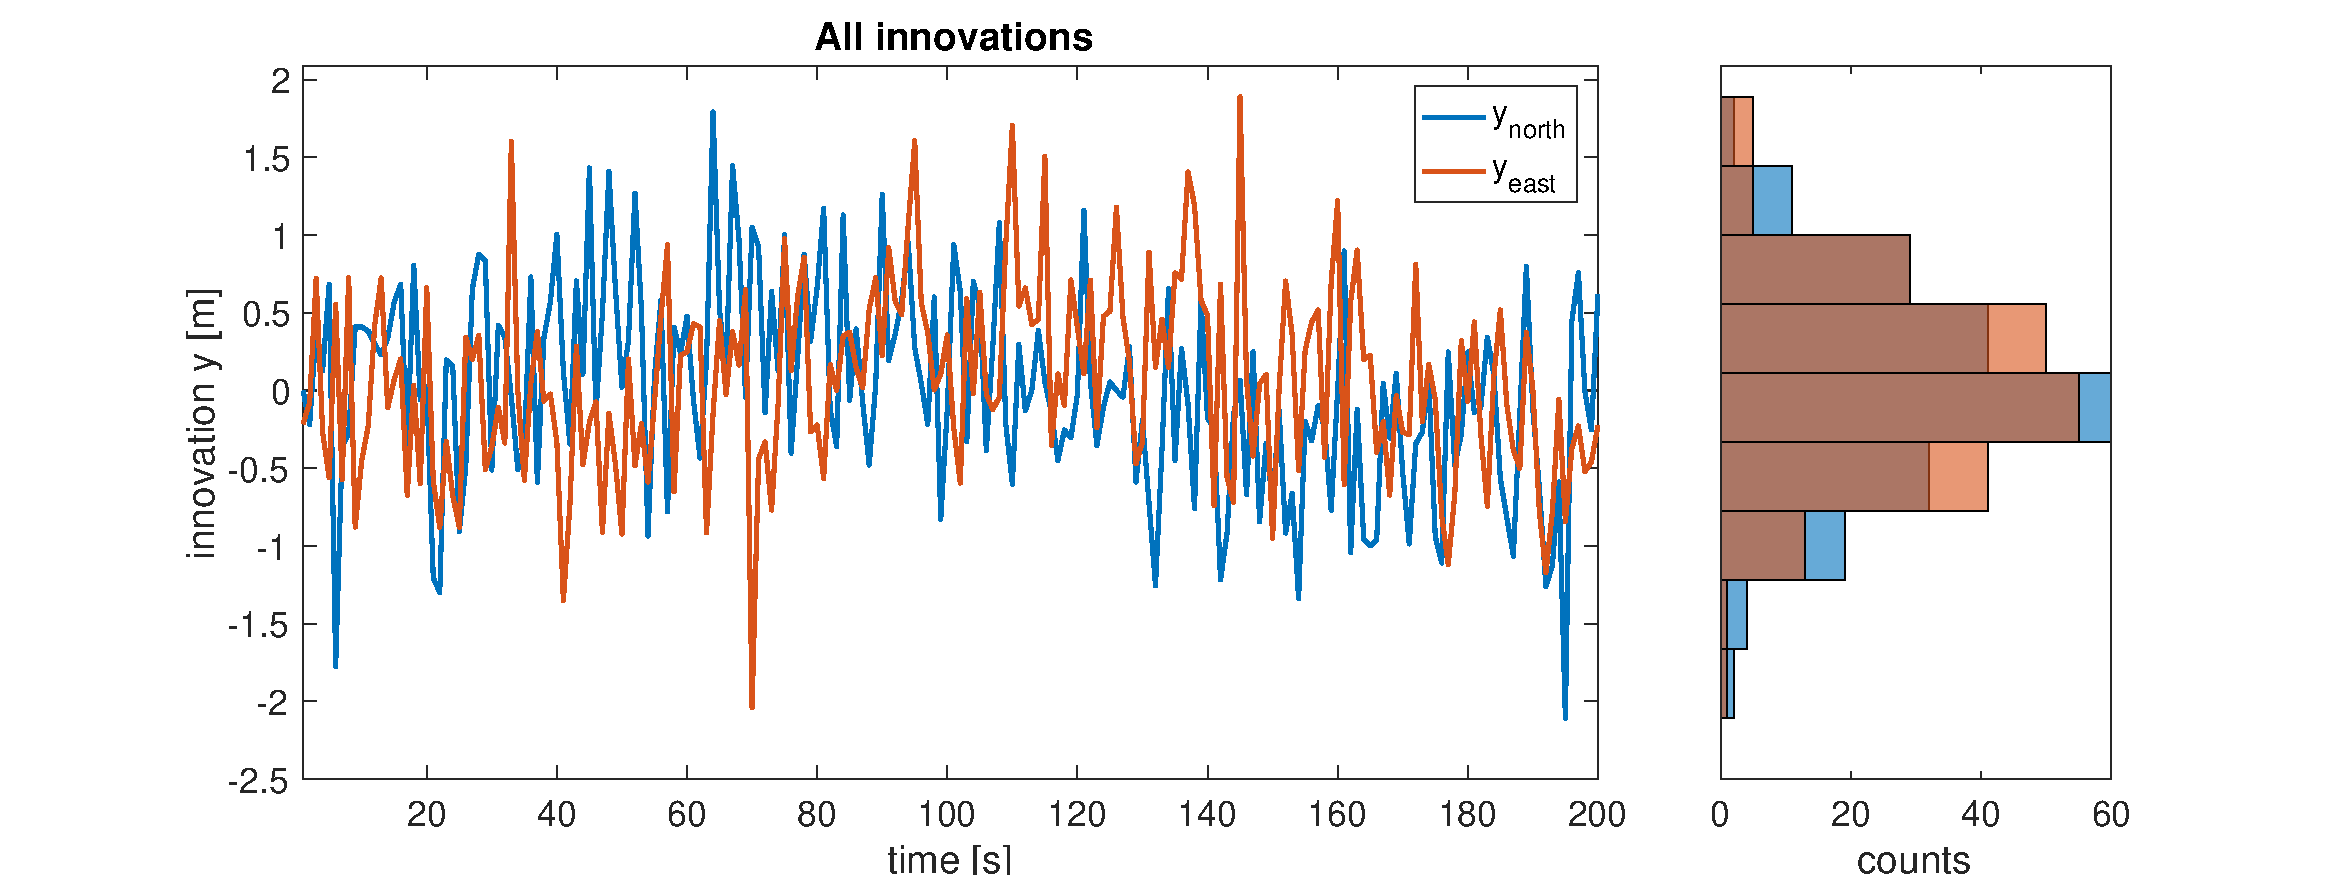
\includegraphics[width=\textwidth]{dt1_smaller_motion_noise/innovation_all}
        \caption{Innovation 10x smaller system noise}
    \end{subfigure}
    ~
    \begin{subfigure}[t]{0.49\textwidth}
        \centering
        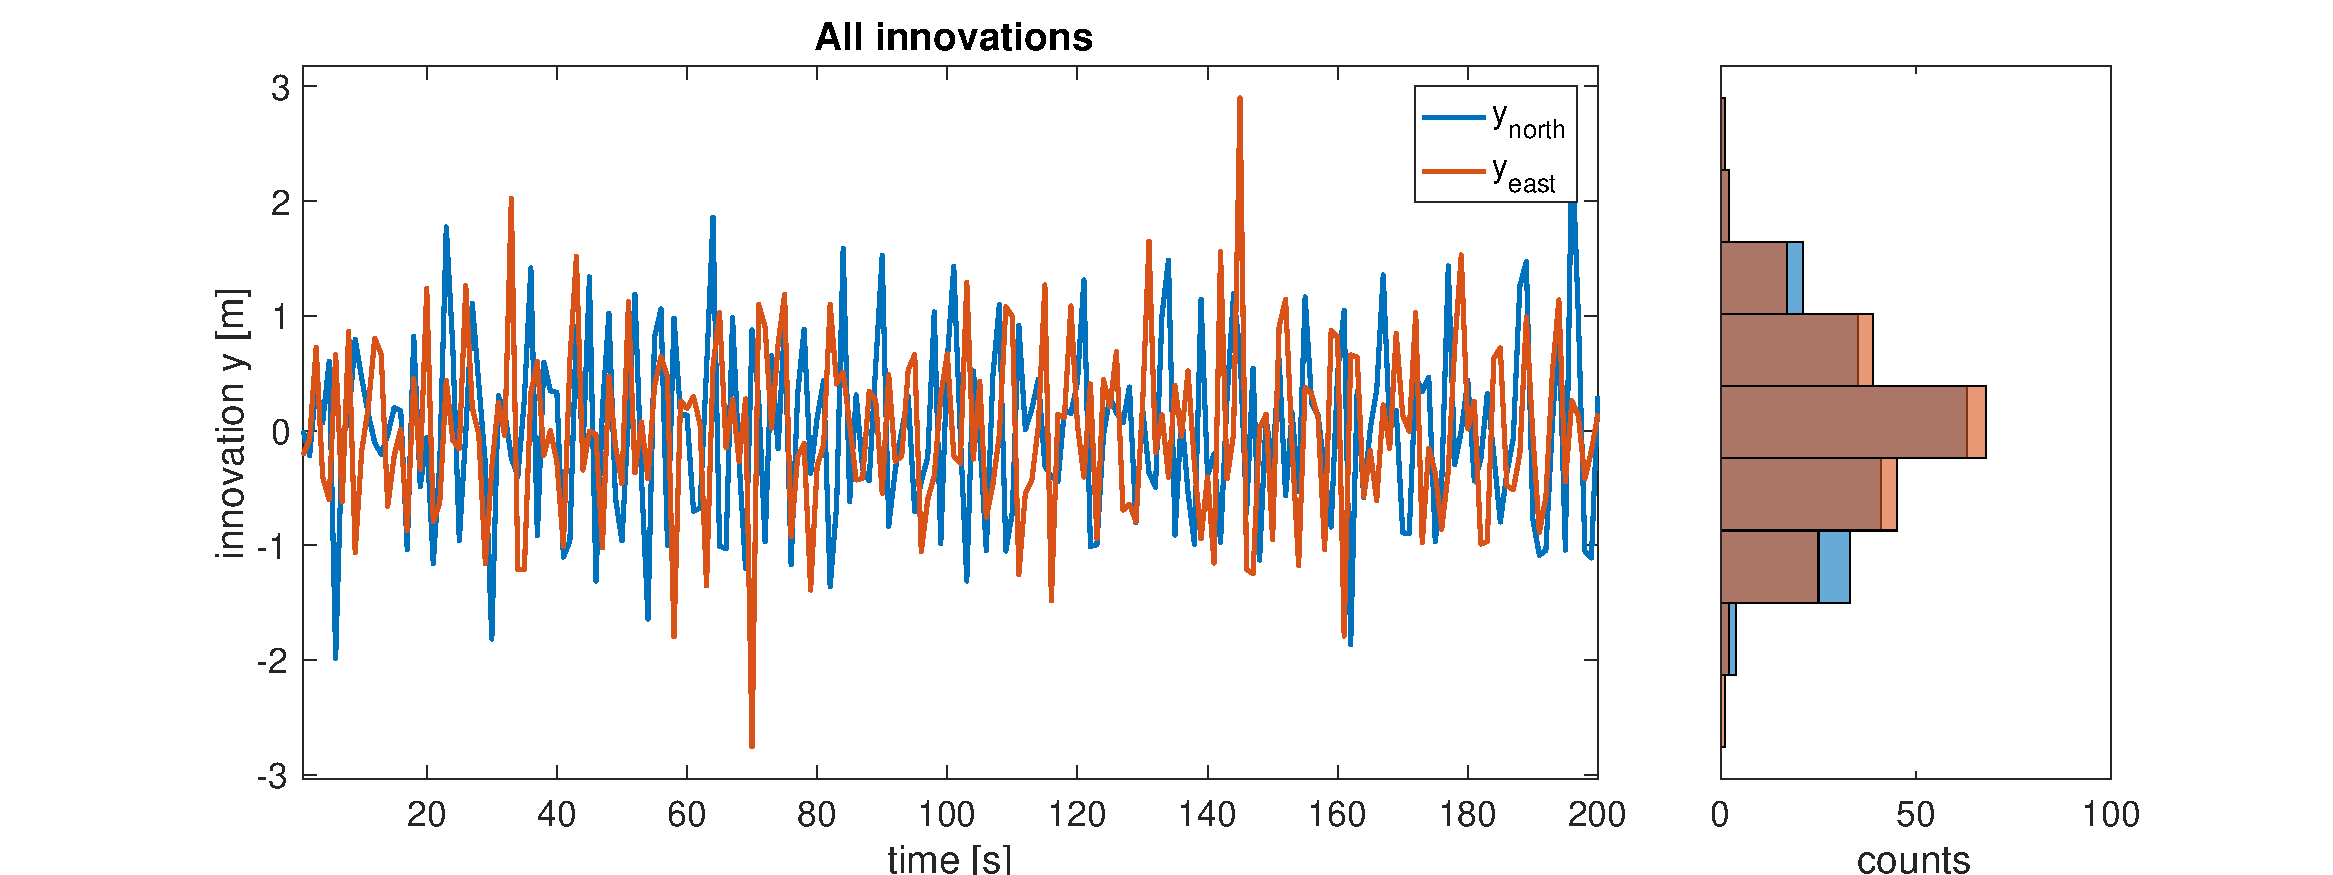
\includegraphics[width=\textwidth]{dt1_bigger_motion_noise/innovation_all}
        \caption{Innovation 10x bigger system noise}
    \end{subfigure}
    ~
    \begin{subfigure}[t]{0.49\textwidth}
        \centering
        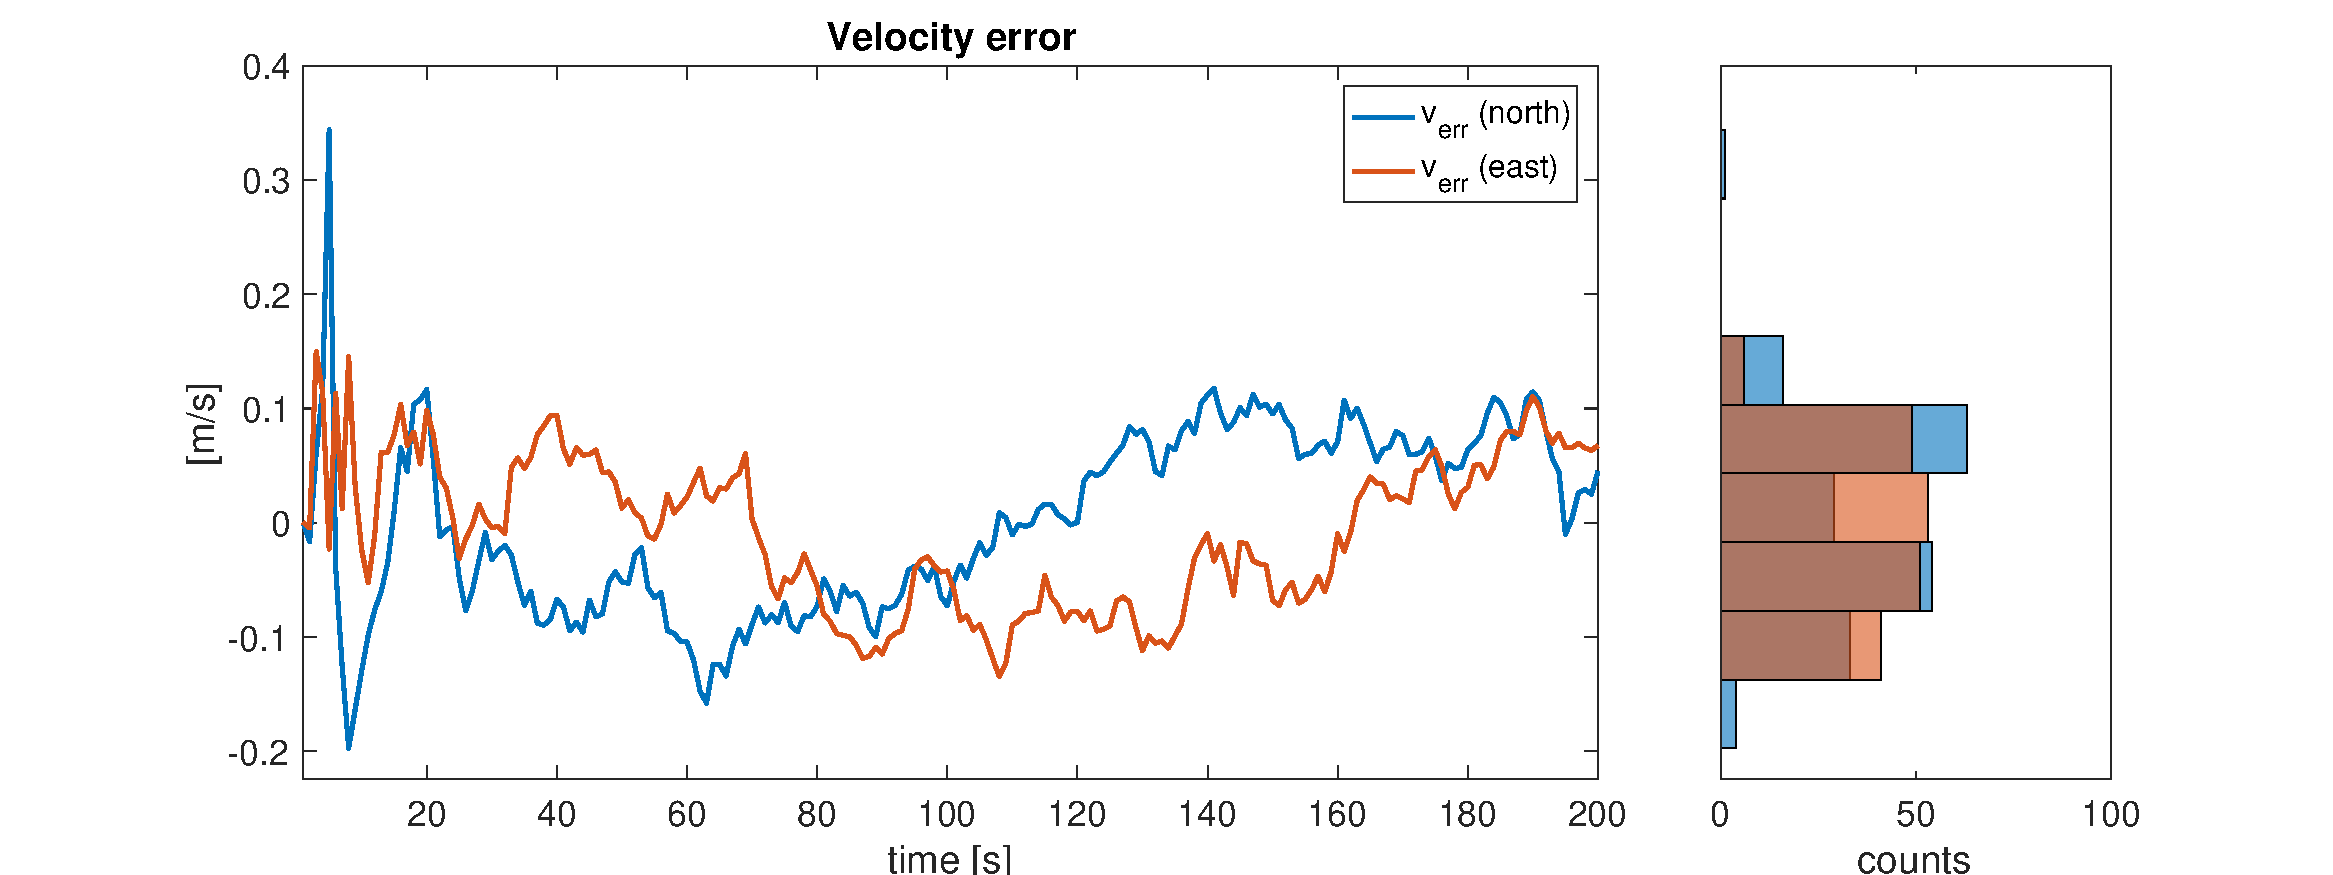
\includegraphics[width=\textwidth]{dt1_smaller_motion_noise/velocity_error}
        \caption{Velocity error 10x smaller system noise}
    \end{subfigure}
    ~
    \begin{subfigure}[t]{0.49\textwidth}
        \centering
        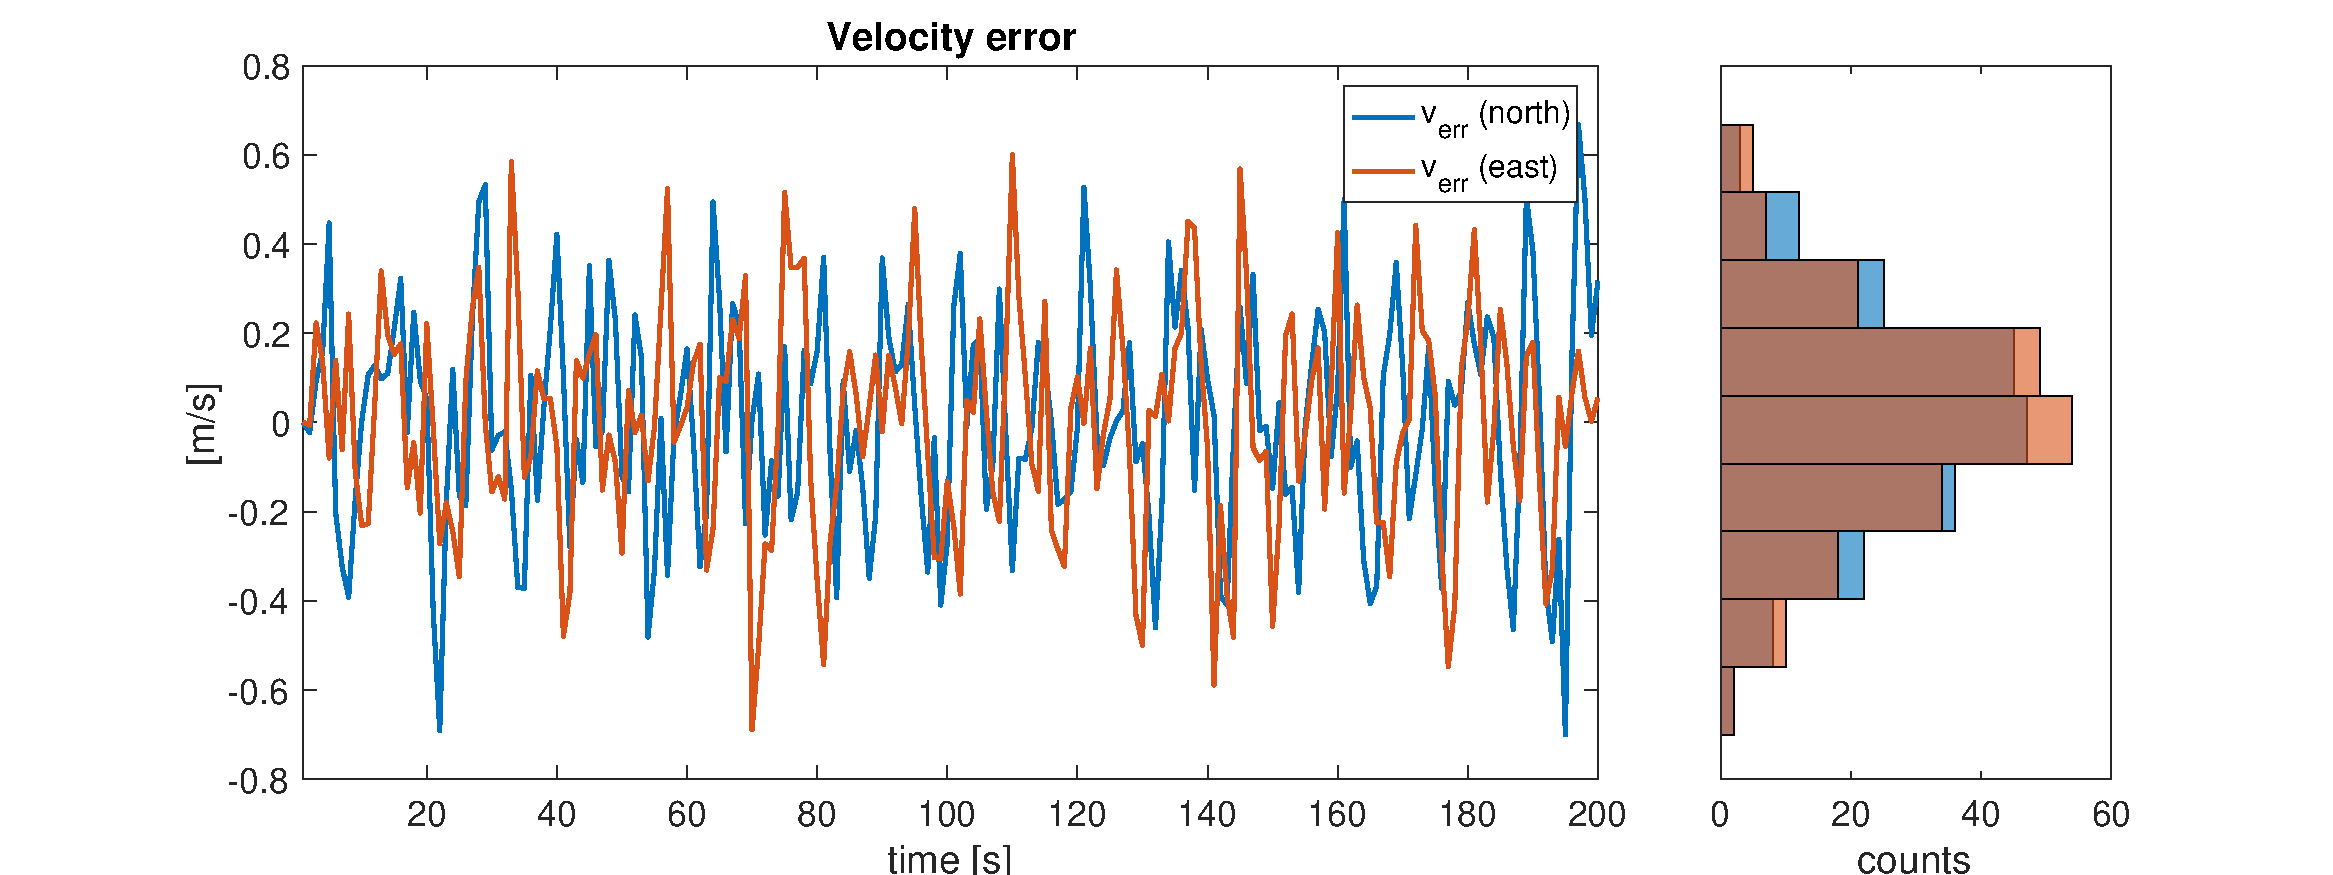
\includegraphics[width=\textwidth]{dt1_bigger_motion_noise/velocity_error}
        \caption{Velocity error 10x bigger system noise}
    \end{subfigure}
    \caption{Results for different system noise levels.}
    \label{fig:traj_motion_noise}
\end{figure}

\newpage
\section*{Code}
\lstinputlisting{../lab8.m}

\end{document}
